\chapter{Deus et Eliseus venerunt in mundum}
\begin{center}
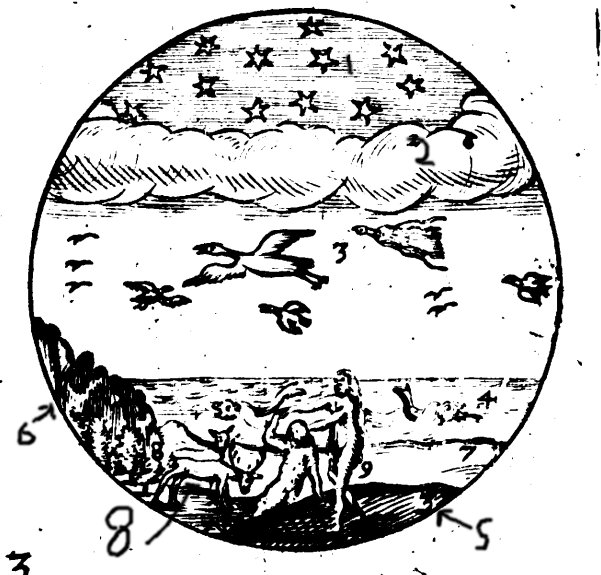
\includegraphics[scale=1.5]{World.png}
\end{center}

\section{Intended Audience}
This is intended for students who have completed Lectio 2 of Latin by the Natural Method and Chapter 3 of Lingua Latina Per Se Illustrata. 336 words are in this chapter.

\section{Text}

Deus accēpit Eliseum et ostendit Eliseō\footnote{\textbf{Eliseō} = To Elisha} mundum. Mundus est rotundus. Deus ostendit Eliseō Caelum(1)\footnote{\textbf{Caelum} = Heaven, Sky}. Caelum habet stēllās\footnote{\textbf{Stēllās, Stēllae} = Stars} . Stēllae habent ignem\footnote{\textbf{Ignis} = Fire} in semetipīs\footnote{\textbf{Semetipīs} = In themselves}.  Moysēs scrīpsit in Genesēō\footnote{\textbf{Genēsis} = The Book of Genesis}, Deus fēcit in caelō lūmināria\footnote{\textbf{Lūmināria} = Lights}. Maius\footnote{\textbf{Maius} = Greater} lūminārium rēgnat diem, et minōra\footnote{\textbf{Minōra} = Lesser} lūmināria rēgnat noctem. Maius Eliseus fuit prophēta. Minus Eliseus est fīlius meus parvus. In nocte sunt stēllae et lūna\footnote{\textbf{Lūna} = The Moon}. Stēllae et Lūna Splendent\footnote{\textbf{Splendent} = They shine} in nocte. Lūna maius lūminārium in nocte. Stēllae minōrēs sunt lūmināria in nocte.\par 
Eliseus vīdit in caelum. "Ecce\footnote{\textbf{Ecce} = Behold}" dīxit Eliseus "Avēs(3)\footnote{\textbf{Avēs} = Birds} volant\footnote{\textbf{Volant} = fly}". Avis\footnote{\textbf{Avis} = Bird} Volat per caelum. Homō(9)\footnote{\textbf{Homō} = Man, Human} est in mundō et venit per\footnote{\textbf{Per} = Through, During} mundum. In caelō sunt nūbēs(2)\footnote{\textbf{Nūbēs} = Clouds}. Avēs volant per nūbēs, et Nūbēs pendent\footnote{\textbf{Pendent} = Hang} in caelō. Chrīstus pependit\footnote{\textbf{Pependit} = He hung} in Cruce\footnote{\textbf{Crux} = The cross} per crucifixiōnem\footnote{\textbf{Crucifixiō} = Crucifixion}. Nūbēs habent umbram\footnote{\textbf{Umbra} = Shadow} in mundō. Eliseus nōn volat, sed venit in mundō. Deus nōn volat, sine locō est. Iēsus volāvit\footnote{\textbf{Volāvit} = He flew}. Deus volāvit in nūbe ignis cum Moyse et Fīliīs\footnote{\textbf{Fīliīs} = With the Sons} Isrāēl. Deus appāruit Moysen et Aarōn et Fīliōs Isrāēl in Monte Horeb in Exodō in Nūbe.\par 
Mundus habet montēs(5)\footnote{\textbf{Montēs} = Montains or Hills}. Mōns\footnote{\textbf{Mōns} = Mountain or hill} est altus. Altissimus\footnote{\textbf{Altissimus} = Highest, most high} Mōns mundī est Mōns Ēvērest. Mundus etiam habet silvās(6)\footnote{\textbf{Silvae, Silvās} = Woods}, quae sunt magnae. Silva habet multās arborēs\footnote{\textbf{Arborēs} = Trees}. Arbor est alta et habet folia\footnote{\textbf{Folia} = Leaves}. Folia sunt parvae et cadunt\footnote{\textbf{Cadunt} = They fall} ex arbore\footnote{\textbf{Ex arbore} = From the tree}. Sub silvā\footnote{\textbf{Sub silvā} = Under the wood} est umbra. Mōns habet umbram. In campō(7)\footnote{\textbf{Campus} = Field} nōn sunt multae arborēs, sed paucae arborēs. Mundus habet campōs, quī habent foenum\footnote{\textbf{Foenum} = Grass}. Animālia(8)\footnote{\textbf{Animal} = Animal}, quae sunt in campō, comedunt\footnote{\textbf{Comedunt} = They eat} foenum. Mōns et silva et campus habent foenum. Foenum est parvus, arbor est magna. Foenum, quod est in campōs, parvum est. Eliseus, fīlius meus parvus, est animal. Deus nōn est animal, sed creātor, cōnservātor, et gubernātor mundī.\par
Mundus habet aquam\footnote{\textbf{Aqua} = Water} in marī\footnote{\textbf{Mare} = Sea}. Mare est locus multae aquae in mundō. Maximum\footnote{\textbf{Maximum} = Biggest} mare est Ōceanus\footnote{\textbf{Ōceanus} = Ocean} Pācificus. In marī piscēs(4)\footnote{\textbf{Piscēs} = Fish} natant\footnote{\textbf{Natant} = They swim}. Piscis natat in aquā, et est animal, et vīvit in aquā. Homō natat in aquā, sed nōn vīvit in aquā. Jonās nōn natāvit et vīxit in marī, quia mortuus\footnote{\textbf{Mortuus} = Dead} fuit in pisce magnō, sīcut in librō Iōnae. Aqua est ūna quattuor\footnote{\textbf{Quattuor} = Four} elementōrum\footnote{\textbf{Elementōrum} = of the elements}. Quattuor elementa\footnote{\textbf{Elementum} = Element} sunt aqua, terra\footnote{\textbf{Terra} = Earth}, āēr\footnote{\textbf{Āer} = Air} et ignis. Mundus plēnus\footnote{\textbf{Plēnus} = Full} est cum quattuor elementīs. 